\documentclass[9pt]{beamer}

\usepackage[utf8x]{inputenc}
\usepackage[romanian]{babel}
\usepackage{xcolor, colortbl}
\usepackage{alltt}
\usepackage{epstopdf}
\usepackage{epsfig}
\usepackage{tikz}
\usetikzlibrary{arrows,positioning}
\usepackage{array, arydshln}
\usepackage{soul}
\usepackage{algorithm,algorithmic}
\usetikzlibrary{matrix,shapes,arrows,positioning}

\floatname{algorithm}{Procedură}
\renewcommand{\algorithmicrequire}{\textbf{Input:}}
\renewcommand{\algorithmicensure}{\textbf{Output:}}

\usepackage{hyperref}
\usepackage{verbatim}
\usepackage{lipsum,graphicx,framed}

\useinnertheme[shadow]{rounded}

\defbeamertemplate*{frametitle}{mytheme}%
{%
    \begin{beamercolorbox}[rounded=true]{title}
      \usebeamerfont{title}\insertframetitle\par%
    \end{beamercolorbox}%
}

\renewenvironment{leftbar}[1][\hsize]%
{%
        \def\FrameCommand%
        {%
             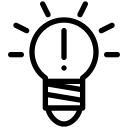
\includegraphics[width=1cm]{figures/idea}%           
             \fboxsep=\FrameSep\colorbox{cyan!5}%
        }%
        \MakeFramed{\hsize#1\advance\hsize-\width\FrameRestore}%
}%
{\endMakeFramed}

\setlength\dashlinedash{0.4pt}
\setlength\dashlinegap{4.5pt}
\setlength\arrayrulewidth{0.2pt}

\newtheorem{concept}{Concept nou}
\newtheorem{demonstratie}{Demonstrație}
\newtheorem{proprietate}{Proprietate}


\makeatletter
\newcommand\SoulColor{%
  \let\set@color\beamerorig@set@color
  \let\reset@color\beamerorig@reset@color}
\makeatother

\mode<presentation>
{ \usetheme{Berlin} }

\PreloadUnicodePage{200}

\title[Time, Clocks, and the Ordering of Events in a Distributed System]{Time, Clocks, and the Ordering of Events in a Distributed System}
\author[Mihai Surdeanu]{\textbf{Mihai Surdeanu}}
\institute[Universitatea Politehnica București]{\textbf{e-Government},\\Facultatea de Automatică și Calculatoare\\Universitatea Politehnica București}

\begin{document}

\AtBeginSection[]
{
  \begin{frame}
    \frametitle{Cuprins}
    \Large{\tableofcontents[currentsection]}
  \end{frame}
}

\setbeamertemplate{frametitle continuation}[from second]

\frame[noframenumbering]{\titlepage}

\addtobeamertemplate{navigation symbols}{}{%
    \usebeamerfont{footline}%
    \usebeamercolor[fg]{footline}%
    \hspace{1em}%
    \insertframenumber/\inserttotalframenumber
}

\section[]{De ce consistența datelor este importantă?}

\begin{frame}{De ce avem nevoie de consistență?}
\begin{itemize}
    \item \Large{Model de consistență}
    \begin{itemize}
		\vskip5pt
		\item O constrângere a unui sistem observabilă de către operațiile aplicației respective.
	\end{itemize}
	\vskip10pt
	\item \Large{Exemple:}
	\begin{itemize}
		\vskip5pt
		\item O memorie x86
		\vskip5pt
		\item O bază de date
	\end{itemize}
	\vskip10pt
\end{itemize}
\centering
\scalebox{0.8} {
    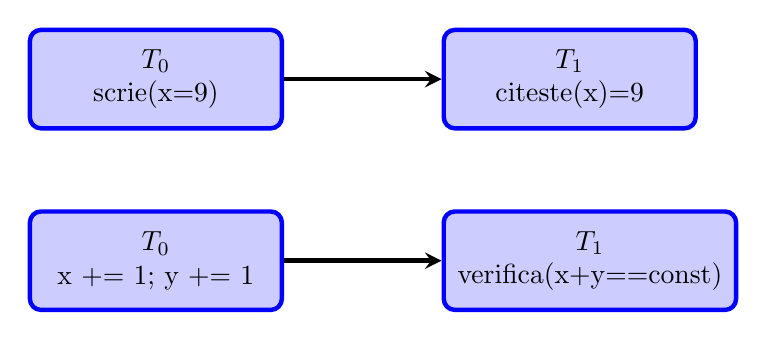
\begin{tikzpicture}[node distance = 1cm] % , auto

    \tikzstyle{construct} = [rectangle,
    ultra thick, rounded corners,
    draw=blue, fill=blue!20, minimum height=1.25cm, minimum width=3.2cm, align=center, inner sep=0.5em]
    \tikzstyle{smallconstruct} = [rectangle,
    ultra thick, rounded corners,
    draw=blue, fill=blue!20, minimum height=1.25cm, align=center, inner sep=0.5em]  \tikzstyle{arrow} = [ultra thick, ->, >=stealth]

    % Nodes
    \node[construct, anchor=mid] (Example1a) {$T_0$\\scrie(x=9)};
    \node[construct, anchor=mid] (Example2a) [below =1cm of Example1a] {$T_0$\\x += 1; y += 1};
    \node[construct, anchor=mid] (Example1b) [right =2cm of Example1a] {$T_1$\\citeste(x)=9};
    \node[construct, anchor=mid] (Example2b) [right =2cm of Example2a] {$T_1$\\verifica(x+y==const)};
    

    % Arrows
    \draw[arrow] (Example1a.east) |- (Example1b.west);
    \draw[arrow] (Example2a.east) |- (Example2b.west);

    \end{tikzpicture}
}
\end{frame}

\begin{frame}{Ce probleme pot apărea?}
\begin{itemize}
    \item \Large{Consistența pe un singur procesor - Probleme:}
    \begin{itemize}
		\vskip5pt
		\item Toate operațiile executate pe un procesor sunt semnate cu un anumit \textit{timestamp} $\rightarrow$
		se cunoaște ordinea de execuție a lor;
	\end{itemize}
	\vskip20pt
	\item \Large{Consistența într-un sistem distribuit - Probleme:}
    \begin{itemize}
		\vskip5pt
		\item Replicarea datelor (caching);
		\vskip5pt
		\item Asigurarea concurenței;
		\vskip5pt
		\item Rezolvarea defectelor;
	\end{itemize}
\end{itemize}
\end{frame}

\begin{frame}{Să mai luăm un exemplu...}
    \begin{figure}
        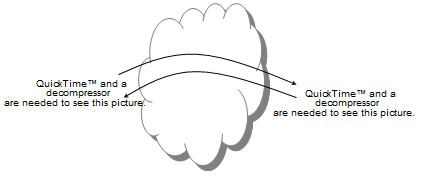
\includegraphics[scale=0.8]{figures/example1}
    \end{figure}
    \begin{description}
        \item[Pasul 1] Fiecare nod are o copie locală
        \vskip5pt
        \item[Pasul 2] Citirea datelor se face din copia locală
        \vskip5pt
        \item[Pasul 3] Rezultatele se trimit către un alt nod, nu se implementează niciun mecanism de așteptare
    \end{description}
\end{frame}

\begin{frame}{Ce se întâmplă în exemplul anterior?}
    \begin{figure}
        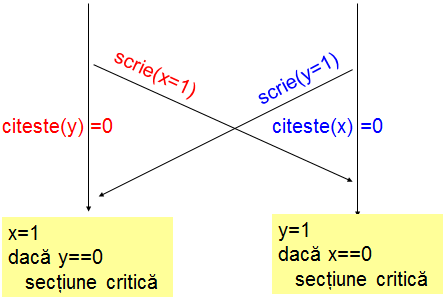
\includegraphics[scale=0.5]{figures/result1}
    \end{figure}
    \vskip5pt
    \centering
	\begin{leftbar}[0.7\textwidth]
        \noindent
        \Large{Fiecare entitate va vedea succesiunea evenimentelor într-o ordine diferită!}
    \end{leftbar}
\end{frame}

\section[]{Asigurarea consistenței în sistemele distribuite}

\begin{frame}{Sistemele distribuite}
\begin{itemize}
    \item \Large{Caracteristici}
    \begin{itemize}
		\vskip5pt
		\item Spațiu diferit pentru fiecare proce în parte
		\vskip5pt
		\item Comunicarea se face prin intermediul mesajelor
		\vskip5pt
		\item Rețeaua poate introduce întârzieri în transmiterea pachetelor
	\end{itemize}
	\vskip10pt
	\item \Large{Cum putem decide în ce ordine s-a petrecut anumite evenimente?}
	\vskip10pt
	\item \Large{Soluții posibile:}
    \begin{itemize}
		\vskip5pt
		\item \SoulColor\hl{Utilizarea unui ceas fizic}
		\vskip5pt
		\item \SoulColor\hl{Sincronicarea cu un server de timp}
	\end{itemize}
\end{itemize}
\end{frame}

\begin{frame}{O altă soluție... Ceasuri logice!}
\begin{itemize}
    \item \Large{Idea de a abandona noțiunea de ceas fizic}
	\vskip10pt
	\item \Large{De multe ori, este suficient să știm ordinea în care anumite evenimente au avut loc}
	\vskip10pt
	\item \Large{\SoulColor\hl{Lamport (1978)} - a introdus noțiunea de \SoulColor\hl{timp logic (virtual)} tocmai pentru a \textit{ordona} anumite evenimente}
\end{itemize}
\end{frame}

\begin{frame}{Ordonarea evenimentelor. Când este necesară?}
\begin{concept}
\Large{Ordonarea evenimentelor este în strânsă legătură cu conceptul de \textbf{cauzalitate}:}
\begin{itemize}
    \vskip10pt
    \item Un eveniment \textbf{a} s-a petrecut înaintea unui eveniment \textbf{b} dacă se poate spune că un eveniment \textbf{a} poate afecta un alt eveniment \textbf{b}.
	\vskip10pt
	\item Dacă evenimentele \textbf{a} și \textbf{b} au loc în cadrul unor procese diferite și nu schimbă date între ele, atunci ordinea nu este importantă.
\end{itemize}
\end{concept}
\end{frame}

\begin{frame}{Relația \textit{s-a petrecut înainte}}
Trebuie să satisfacă următoarele 3 condiții:
    \begin{columns}
        \begin{column}[c]{0.70\textwidth}
            \begin{description}
            \item[$C_1$] Fiind date două evenimente \textbf{a} și \textbf{b} în cadrul aceluiași proces, \textbf{a} precedându-l pe \textbf{b}, atunci $a \rightarrow b$.
            \vskip5pt
            \item[$C_2$] Dacă evenimentul \textbf{a} reprezintă trimiterea unui mesaj, iar \textbf{b}-ul recepționarea lui (de către un proces diferit) atunci $a \rightarrow b$.
            \vskip5pt
            \item[$C_3$] \textit{(Tranzitivitate)} $a \rightarrow b$ și $b \rightarrow c$ $\Rightarrow$ $a \rightarrow c$.
        \end{description}
        \end{column}
        
        \begin{column}[c]{0.50\textwidth}
            \begin{figure}
            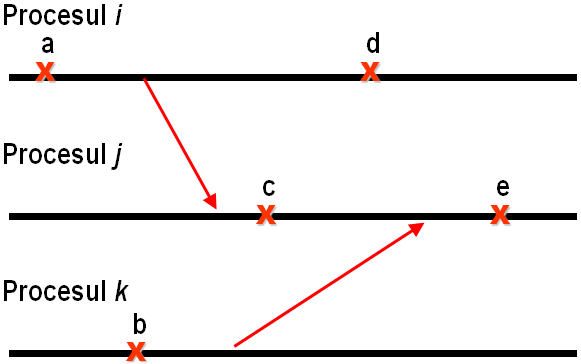
\includegraphics[scale=0.3]{figures/happen1}
            \caption{Exemplu de relații între procese}
            \end{figure}
        \end{column}
    \end{columns}
\vskip10pt
\centering
\Large{Care sunt relațiile pe care le obținem?\\ Relația curentă este de fapt doar o ordonare parțială.}
\end{frame}

\section[]{Ceasuri logice. Ordonarea parțială a evenimentelor}

\begin{frame}{Ceasuri logice. Elemente introductive.}
\begin{concept}
\Large{Definim clock condition ca fiind:}\\
\begin{center}
dacă $a \rightarrow b$ atunci $C_{<a>}$ $<$
$C_{<b>}$
\end{center}
împreună cu următoarele două sub-condiții:
\begin{itemize}
    \vskip10pt
    \item dacă \textbf{a} și \textbf{b} sunt evenimente în procesul $P_i$ și \textbf{a} are loc înaintea lui \textbf{b}, atunci $C^i_{<a>}$ $<$ $C^i_{<b>}$
	\vskip10pt
	\item dacă \textbf{a} reprezintă trimiterea unui mesaj de $P_i$ și \textbf{b} reprezintă recepționarea lui de $P_j$ atunci $C^i_{<a>}$ $<$ $C^j_{<b>}$
\end{itemize}
\end{concept}
\end{frame}

\begin{frame}{Exemplu de sistem}
\centering
\begin{figure}
    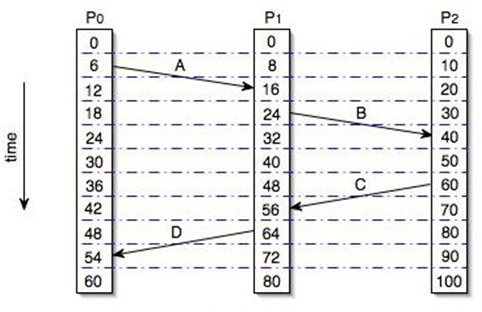
\includegraphics[scale=0.6]{figures/happen2}
    \caption{Trei procese cu propria logică de menținerea a ceasului intern}
\end{figure}
\end{frame}

\begin{frame}{Reguli de implementare al unui astfel de sistem}
Următoarele reguli trebuie să fie implementate:
    \begin{columns}
        \begin{column}[c]{0.70\textwidth}
            \begin{description}
            \item[$R_1$] Între două evenimente succesive ale unui proces se apelează $incrementeaza(C_i)$
            \vskip5pt
            \item[$R_2$] Dacă \textbf{a} este trimiterea unui mesaj \textbf{m} atunci \textbf{m} conține un timestamp $T_m$ unde $T_m$=$C^i_{<a>}$
            \begin{itemize}
            \vskip5pt
            \item Când un proces $P_k$ primește mesajul m trebuie să seteze $C_k$ astfel încât:\\ $T_{curent} \leq T_m< C_k$
            \end{itemize}
            \end{description}
        \end{column}
        
        \begin{column}[c]{0.50\textwidth}
            \begin{figure}
            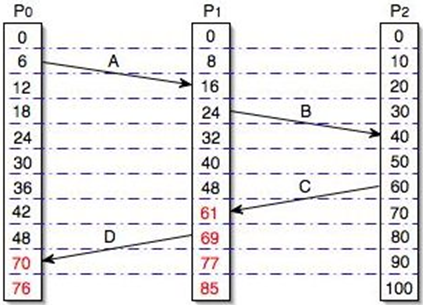
\includegraphics[scale=0.4]{figures/happen3}
            \caption{Funcționarea algoritmului}
            \end{figure}
        \end{column}
    \end{columns}
\vskip10pt
\centering
\Large{Care este corespondeța între regulile pe care le avem și condițiile de pe slide-urile anterioare?}
\end{frame}

\section[]{Ordonarea completă a evenimentelor - Distributed Resource Allocation}

\begin{frame}{Definirea unei ordonări complete}
\begin{concept}
\Large{Putem defini o ordine completă asupra unui set de evenimente $a \Rightarrow b$:}\\
\begin{center}
$C^i_{<a>}<C^j_{<b>}$\\sau\\
$C^i_{<a>}=C^j_{<b>}$ și $P_i?P_j$ unde \textit{?} este o relație arbitrară de ordonare între procese
\end{center}
\end{concept}
\vskip15px
\Large{În acest moment se poate crea un algoritm - \textit{Distributed Resource Allocation} care să permită rezolvarea unei probleme mutual exclusive.}
\end{frame}

\begin{frame}{Distributed Resource Allocation}
\Large{Algoritmul trebuie să satisfacă următoarele \textit{3 condiții}:}
    \begin{description}
        \item[$C_1$] Un proces care a pus la dispoziție resursa respectivă trebuie să o elibereze înainte de a putea fi oferită altui proces.
        \vskip5pt
        \item[$C_2$] Cererile pentru resursa respectivă trebuie să fie oferite în ordinea în care au fost efectuate.
        \vskip5pt
        \item[$C_3$] Dacă fiecare proces care acordă resursa o eliberează în cele din urmă, se poate spune că fiecare cerere oferită.
    \end{description}
\end{frame}

\begin{frame}{Distributed Resource Allocation (II)}
\Large{La baza implementării algoritmului stau \textit{5 reguli}:}
    \begin{description}
        \item[$R_1$] Pentru a cere o resursă, $P_i$ trimite un mesaj $T_m:P_i$ \textit{requests resource} de tip broadcast și adaugă mesajul respectiv în propria coadă.
        \vskip5pt
        \item[$R_2$] La primirea unui astfel de mesaj, procesul $P_k$ îl plasează în propria coadă de cereri și trimite un ack - \textit{OK reply} către $P_i$.
        \vskip5pt
        \item[$R_3$] Pentru eliberarea resursei, $P_i$ scoate orice mesaj de tipul $T_m:P_i$ \textit{requests resource} din coada internă și trimite un mesaj de tip broadcast - timestamped $P_i$ \textit{releases resource}.
        \item[$R_4$] Când procesul $P_k$ primește un mesaj de tipul \textit{releases resource} scoate mesajele $T_m:P_i$ \textit{requests resource} din coada proprie.
    \end{description}
\end{frame}

\begin{frame}{Distributed Resource Allocation (III)}
    \begin{description}
        \item[$R_5$] Resursa $P_i$ este oferită atunci când:
        \begin{enumerate}
        \item Există un mesaj de tipul $T_m:P_i$ \textit{requests resource} în coada internă ce a avut loc înainte de orice altă cerere definită de relația "$\Rightarrow$".
        \item $P_i$ a primit un mesaj de la un alt proces timestamped mai târziu de $T_m$.
        \end{enumerate}
    \end{description}
    \centering
    \begin{columns}
        \column{0.5\textwidth}
        \begin{figure}[h]
            \centering
            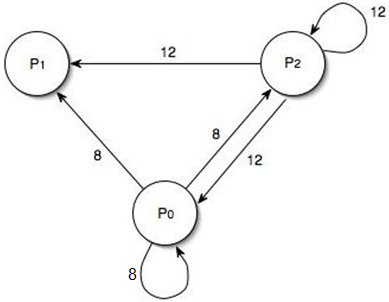
\includegraphics[scale=0.4]{figures/dra1}
            \caption{$P_0$ și $P_2$ cer acces simultan la o resursă}
            \label{fig:res1}
        \end{figure}
        \column{0.5\textwidth}
        \begin{figure}[h]
            \centering
            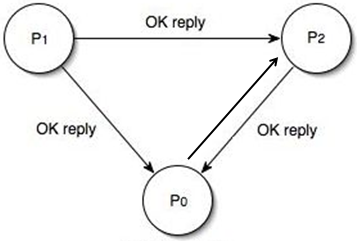
\includegraphics[scale=0.4]{figures/dra2}
            \caption{$P_0$ primește acces la resursa respectivă. De ce?}
            \label{fig:res2}
        \end{figure}
    \end{columns}
\end{frame}

\begin{frame}{Posibile anomalii}
\Large{În anumite condiții, algoritmul prezentat pentru sistemele distribuite, poate conduce la diverse anomalii:}
    \begin{itemize}
        \vskip5pt
        \item dictarea de schimbări la nivelul telefonului
        \vskip5pt
        \item failure-uri la nivelul unui sistem - al unui proces
        \vskip5pt
        \item în principiu tot felul de interacțiuni cu mediul extern
    \end{itemize}
\vskip10pt
\centering
\huge{\rm{Trebuie să folosim ceasuri fizice!}}
\end{frame}

\section[]{Integrarea ceasurilor fizice}

\begin{frame}{Ceasuri fizice}
\begin{itemize}
    \item Fie $C_i(t)$ valoarea aratată de ceasul $C_i$ la momentul de timp $t$.
    \vskip5pt
    \item Presupunem că $C_i(t)$ este o funcție diferențială în funcție de timp $\frac{dC_i(t)}{dt}\approx1$, rata cu care ceasul $C_i$ rulează în timp
    \vskip10pt
\end{itemize}
\begin{description}
    \item[$PC_1$] Ținând cont de toate aceste aspecte putem presupune că există o constantă $\alpha$ pentru care există relația:\\
    $\lvert\frac{dC_i(t}{dt}-1\rvert<\alpha$. ($\alpha<10^{-6}$ pentru ceasurile cu quartz)
\end{description}
\begin{itemize}
    \item Ce ne propunem? Răspuns: $C_i(t)\approx C_j(t),\forall i,j,t$. De aici se poate deduce:
    \vskip10pt
\end{itemize}
\begin{description}
    \item[$PC_2$] $\exists$ $\epsilon$, $\forall i,j$ astfel încât: $\lvert C_i(t)-C_j(t)\rvert<\epsilon$
\end{description}
\begin{itemize}
    \item În aceste condiții când se poate produce o anomalie?
\end{itemize}
\end{frame}

\begin{frame}{Ceasuri fizice (II)}
\begin{itemize}
    \item În continuare, să presupunem că $\mu$ reprezintă cel mai mic timp de transmitere a unui mesaj între două procese.
    \vskip5pt
    \item Pentru a evita apariția de comportamente anormale, va trebui să fie îndeplinită condiția: $C_i(t+\mu)-C_j(t)>0$.
    \vskip5pt
    \item Folosind $PC_1$ se va obține: $C_i(t+\mu)-C_j(t)>(1-\alpha)\mu$.
    \vskip5pt
    \item Pentru ca $PC_1$ să fie adevărată este necesar: $\epsilon\leq(1-\alpha)\mu$.
    \vskip10pt
\end{itemize}
\end{frame}

\begin{frame}{Ceasuri fizice - Implementare}
Regulile 1 și 2 de la ceasurile virtuale pot fi acum extinse astfel:
    \begin{description}
        \item[$R_1'$] Dacă $P_i$ nu primește un mesaj la momentul de timp $t$, atunci $dC_i(t)/dt>0$
        \vskip5pt
        \item[$R_2'$] Dacă $P_i$ trimite un mesaj atunci acesta va avea timestampul $T_m=C_i(t)$. La recepționarea unui mesaj $m$ la momentul de timp $t'$ procesul $P_j$ va seta $C_j(t')=max(C_j(t'),T_m+\mu_m)$
    \end{description}
\end{frame}

\section[]{Concluzii și posibile îmbunătățiri}

\begin{frame}{Concluzii}
\begin{enumerate}
    \item \textbf{Ceasurile virtuale} pot fi utilizate cu succes în ordonarea evenimentelor ce au loc într=in sistem distribuit.
    \vskip5pt
    \item \textbf{Ordonarea parțială} a evenimentelor poate fi extinsă la o ordonare completă pentru a rezolva diverse probleme de sincronizare.
    \vskip5pt
    \item \textbf{Ordonarea completă} este oarecum arbitrată, nici ea nu este unică și poate cauza diverse anomalii comportamentale.
    \item Aceste anomalii pot fi prevenite dacă se introduce noțiunea de \textbf{timp fizic} în sistemul nostru.
\end{enumerate}
\end{frame}

\begin{frame}{\textit{Extra Slide} - Probleme cu această soluție}
\begin{enumerate}
    \item O problemă cu această soluție este faptul că pot exista o pereche de evenimente distincte $(a,b)$ care să aibă același timestamp Lamport. Pentru a realiza această problemă va trebui să ținem cont și de identitatea procesului la realizarea ordonării totale.
    \vskip5pt
    \item O altă problemă cu această soluție este că dacă $C_{<a>} < C_{<b>}$ atunci nu se poate stabili și că $a \rightarrow b$. Altfel spus nu se poate determina care perechi de evenimente sunt cauzale și care nu (evenimentele cauzale sunt văzute de fiecare node din sistem în aceeași ordine).
    \vskip5pt
    \item Rezolvarea acestor probleme s-a realizat prin introducerea unor \textbf{ceasuri vectoriale}.
\end{enumerate}
\centering
\begin{figure}
    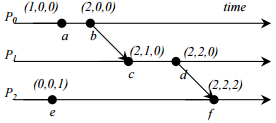
\includegraphics[scale=0.5]{figures/vector}
    \caption{Cum arată mesajele trimise folosind ceasuri vectoriale.}
\end{figure}
\end{frame}

\begin{frame}{Referințe \& Întrebări}
  \begin{columns}
    \begin{column}[c]{0.70\textwidth}
        \begin{thebibliography}{10}    
        \beamertemplatebookbibitems
            \bibitem{Reference1}
            L.~Lamport
            \newblock {\em Time, Clocks, and the Ordering of Events in a Distributed System}.
            \newblock Massachusetts Computer Associates, Inc. - July 1978.
        \beamertemplatearticlebibitems
            \bibitem{Reference2}
            L.~Jinyang
            \newblock {\em Ordering of events in Distributed Systems \& Eventual Consistency}.
            \newblock Online presentation, May 2012.
        \beamertemplatearticlebibitems
            \bibitem{Reference3}
            Y.~Kantor
            \newblock {\em Lamport Algorithm}.
            \newblock Online presentation, June 2009.
        \end{thebibliography}
    \end{column}

    \begin{column}[c]{0.30\textwidth}
      \begin{figure}
        
\includegraphics[scale=0.2]{figures/question}
      \end{figure}
    \end{column}
  \end{columns}
\end{frame}

\end{document}